% \chapter*{\Huge Big Title Here}
% \addcontentsline{toc}{chapter}{Big Title Here}  % Add to TOC if needed

\chapter{Foundational structures: diagnosis and prognosis experts} % Main chapter title
%---------------------------------------------------------------------------------------
%	SECTION 
%----------------------------------------------------------------------------------------

\section{Introduction}
%-----------%-----------
%	SOUS-SECTION 
%-----------%-----------
\subsection{Contextual background}

Ultrasonography, a common diagnostic modality in both human and veterinary medicine, is particularly valued for its non-invasiveness, portability, and rapid assessment capabilities. Specifically, in veterinary medicine, thoracic ultrasonography (TUS) is extensively employed as a quick, accurate, and practical method for diagnosing lung lesions associated with respiratory diseases such as Bovine Respiratory Disease (BRD). It provides an immediate, real-time assessment of lung pathology without the limitations of other imaging techniques such as radiography or computed tomography, which involve high costs, radiation exposure, and require specialized facilities and sedation or anesthesia \cite{ollivett_-farm_2016}. Pulmonary ultrasound videos provide a direct view of the lung tissue, making them highly relevant for assessing the severity of respiratory diseases like BRD. TUS can accurately identify critical pathological features associated with disease severity and prognosis, including consolidated lung tissue, lobar pneumonia, abscess formation, and pleural effusion. In feedlot cattle, Timsit et al. (2019) \cite{timsit_association_2019} demonstrated that the maximal depth and area of lung consolidation measured at the time of bronchopneumonia diagnosis using TUS were significantly associated with an increased risk of disease relapse and negatively impacted animal growth performance. \cite{timsit_association_2019} Interpreting ultrasound images poses challenges even for skilled experts due to inherent limitations of ultrasonography. Ultrasound images typically appear as noisy, black-and-white visuals that provide limited detail, capturing only two-dimensional representations of tissue shapes and echo patterns. The presence of artifacts such as comet tails or reverberations, as well as the subjective nature of differentiating between subtle variations in lung tissue echogenicity, further complicates the interpretation of lung ultrasounds. Additionally, lung lesions must reach the pleural surface to become visible ultrasonographically, limiting the detection of deeper pulmonary pathology. Despite these limitations, thoracic ultrasonography remains highly valuable due to its real-time diagnostic capability, portability, and practical utility in large-animal field settings, offering immediate insights into disease severity and prognosis when assessing BRD outbreaks on-farm.


%une des limitations aussi de ce type d'observations et qui motive également à aller vers du processing multimodal d'observations est que les lésions ou artéfacts vue dans les poumons sont souvent indicateurs d'évenements tardifs ? Ultrasound imaging can only detect lung lesions that extend to the pleural surface, meaning lesions deeper within the lung parenchyma or isolated deep within the lung cannot be visualized effectively. Thus, lesions entirely surrounded by aerated lung tissue, such as deep lung abscesses or lesions not reaching the pleural surface, may go undetected using TUS (cf ollivett) Not all lung lesions visualized by TUS correlate equally with clinical outcomes. While maximal depth and area of lung consolidation detected by ultrasound strongly predict negative outcomes, certain observed features, like comet-tail artifacts or minimal pleural effusion, may have limited or no prognostic relevance, reducing the comprehensive clinical utility of ultrasound alone in certain contexts (timsit, 2019).

A stochastic mechanistic model, developed by Picault et al. (2022) \cite{picault_modelling_2022}, was created to study BRD propagation and evaluate the impact of farming practices, including pen size, risk levels of cattle, and antimicrobial treatments (individual versus collective metaphylaxis). The motivation behind this model was the need to explore optimal BRD management practices in different farming conditions, specifically assessing the balance between disease control effectiveness and antimicrobial usage. Twelve scenarios, reflecting various fattening systems characterized by differences in pen size (small pens of 10 animals vs. large pens of 100 animals), risk levels (low, high, and high risk mitigated by preventive antimicrobial treatment), and treatment protocols (individual or collective metaphylaxis), were evaluated. Model parameters were calibrated using existing empirical data and relevant veterinary literature. Results demonstrated that BRD occurrence, severity, and mortality were predominantly influenced by risk level and pen size. Large pens and higher risk levels consistently resulted in increased severity and higher mortality rates. The model also emphasized the effectiveness of collective antimicrobial treatments during fattening periods, particularly in large pens with high-risk scenarios, by significantly reducing disease severity and mortality despite the associated increase in antimicrobial usage. Conversely, implementing measures to reduce risk at pen formation provided the best overall outcomes, effectively minimizing both antimicrobial usage and cumulative disease duration. However, this mechanistic model had previously been mostly calibrated from existing veterinary literature, leading to uncertainties regarding its practical and explanatory utility with real-world veterinary data and highlighting the importance of future validation with empirical datasets to enhance its practical applicability.

\subsection{Originality and objective of this Work}

\subsubsection*{diagnosis and prognosis expertise}

The SEPTIME project has enabled the collection of empirical data addressing critical knowledge gaps in Bovine Respiratory Disease (BRD), providing diverse datasets captured at varying temporal frequencies. Lung ultrasound videos (LUS) were recorded and employed due to its rapid, non-invasive capability for diagnosing respiratory conditions. Throughout the project's duration, lung ultrasound videos were recorded. Although the dataset assembled within this project is extensive, the analysis presented in this chapter utilizes only a subset due to the limited number of observations available. The labelled observations from these LUS videos represent a valuable foundation for evaluating and benchmarking various modelling methods. However, the primary challenge addressed in this work pertains to the limited quantity of observations available at the time of analysis, which constrains the ability to establish robust long-term prognostic insights.

\begin{figure}
  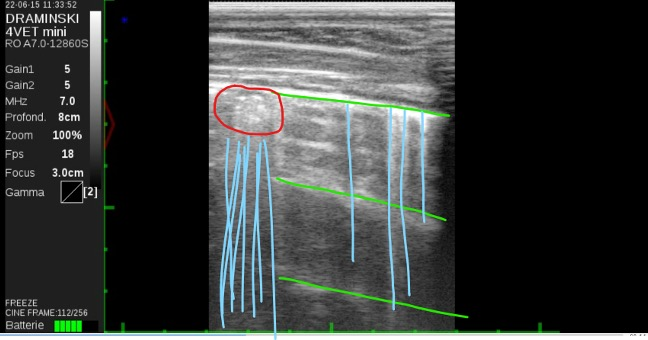
\includegraphics[width=\linewidth]{figures/chap2/annotated_ultrasound.jpg}
  \caption{Pulmonary ultrasound}
  \label{fig:ultrasound}
\end{figure}
\newpage

Achieving accurate and consistent results requires significant operator skill, training, and a systematic examination technique based on anatomical and ultrasonographic landmarks (fig \ref{fig:ultrasound}). Variations in operator skill levels can result in differing degrees of diagnostic accuracy and reliability, making standardized training and experience crucial for correct implementation


% Achieving accurate and consistent results requires significant operator skill, training, and a systematic examination technique based on anatomical and ultrasonographic landmarks. Variations in operator skill levels can result in differing degrees of diagnostic accuracy and reliability, making standardized training and experience crucial for correct implementation

This study therefore addresses two scientifically complementary research questions, directly inspired by contextual gaps and illustrated by our methodological contributions:

\paragraph{To what extent can deep learning reliably automate short-term diagnosis using limited, and context-specific observational data from sensors, such as lung ultrasounds ?} Unlike previous methods relying on manually extracted lesion characteristics \cite{timsit_association_2019}, our objective is to evaluate the extent to which deep learning architectures can autonomously derive high-level semantic representations from lung ultrasound videos.  We could then use this diagnosis expert to perform occasional diagnosis at different observation dates, this handles the need of a lot of data and could still provide first hand description of the health status (fig \ref{fig:chap2-question1}). We hypothesize that capturing the spatio-temporal patterns present in ultrasound videos through deep learning architectures can significantly enhance diagnostic robustness, particularly in field conditions where traditional manual lesion characterization is limited by subjectivity and variability. It might be lesion or it could another artefacts that the human eye wouldn't easily detect. This "sensor-to-diagnosis" automation could support veterinarians by offering immediate and objective assessments of animal health, providing valuable insight into the clinical state without extensive manual feature extraction or prolonged observational periods. Importantly, this approach could be practically deployed as a rapid and non-invasive technique to perform regular health monitoring, allowing veterinarians to obtain explicit, short-term descriptions of animal health status.

\begin{figure}
  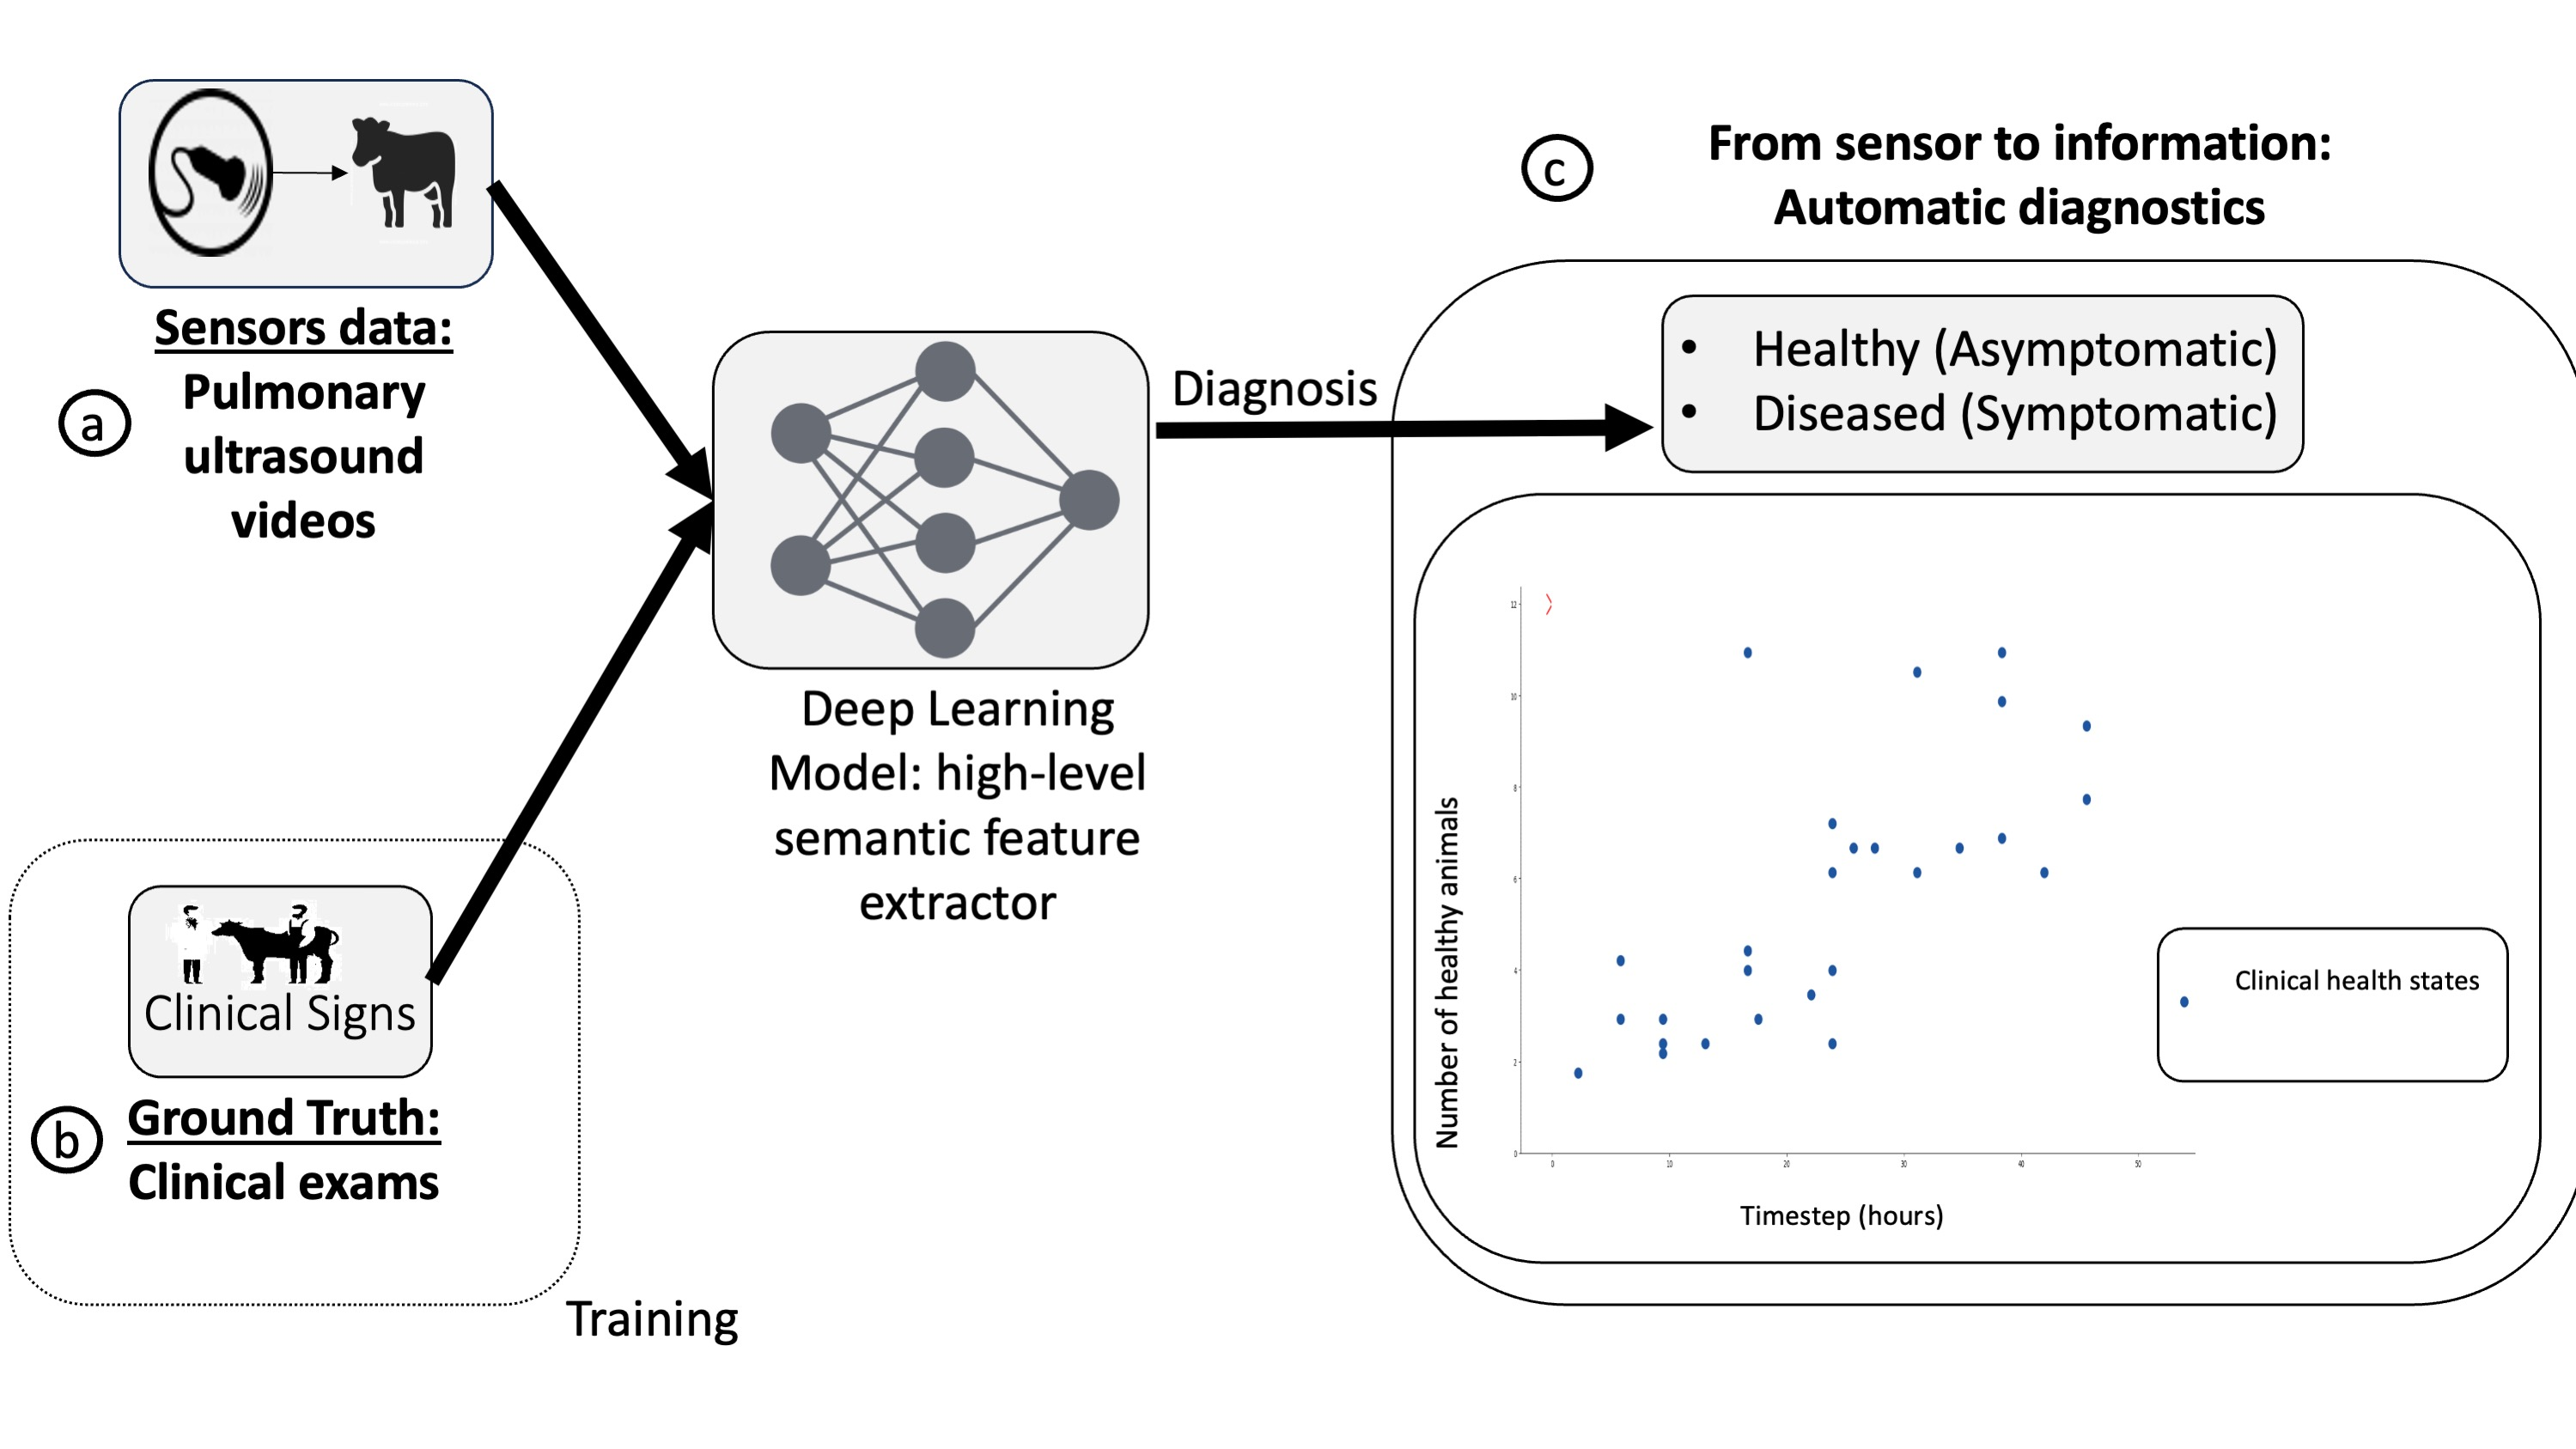
\includegraphics[width=\linewidth]{figures/chap2/chap1-question1.jpg}
  \caption{Can we use deep learning to automated the diagnosis at occasional date points using the limited available observations from sensors ?}
  \label{fig:chap2-question1}
\end{figure}
\newpage
    
\paragraph{Can mechanistic epidemiological models be parametrized using empirical veterinary observations to provide accurate explanatory long-term predictions for BRD ?} The previously established stochastic mechanistic model for BRD propagation \cite{picault_modelling_2022} was calibrated using theoretical assumptions rather than empirical veterinary observations, limiting its practical validation. In this work, we investigate whether empirical veterinary assessments considered ground truth, collected at limited temporal intervals and sparse frequency, can effectively parametrize a mechanistic epidemiological model to reliably predict BRD dynamics. Since daily health observations can be logistically challenging and costly in practice, we aim to assess whether accurate modelling can still be achieved by fitting the model to sparse empirical observations, allowing it to explicitly reconstruct disease dynamics and clinical states even on unobserved days (fig \ref{fig:chap2-question2}). Anything can happen in between the points, we could rely on the theoretical knowledge embedded in mechanistic models to explicit and give us evidence-based insights.


\begin{figure}
  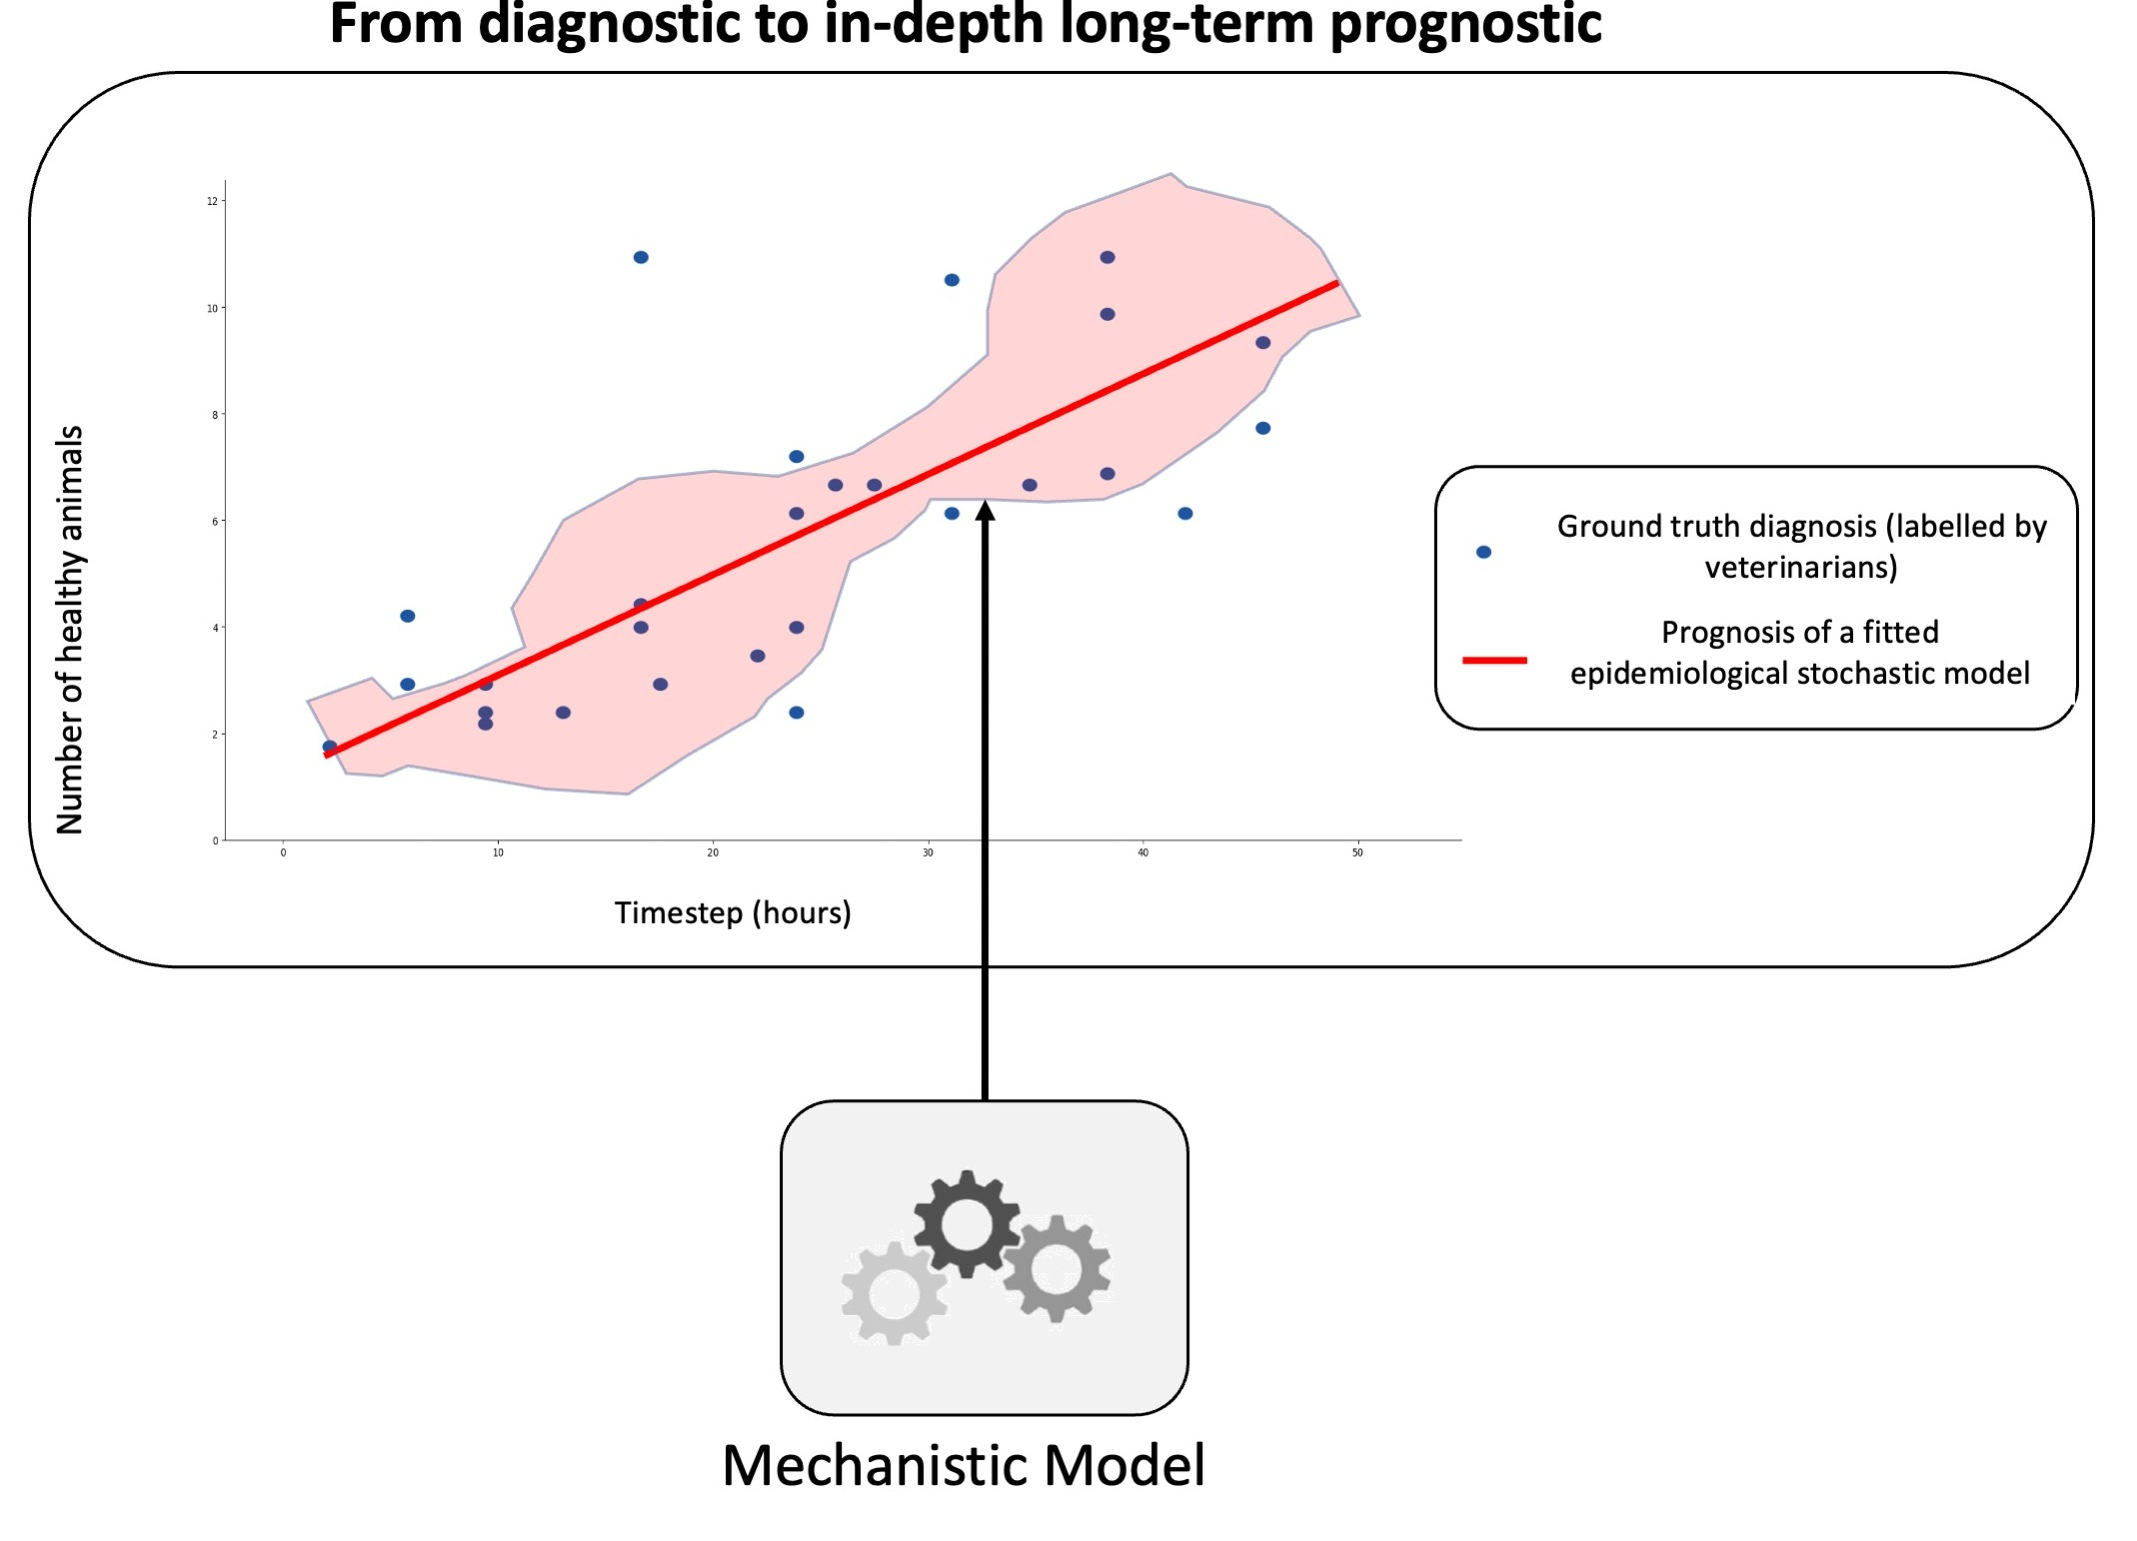
\includegraphics[width=\linewidth]{figures/chap2/chap1-question2.jpg}
  \caption{Can a mechanistic model for BRD be fitted to real-wolrd observations from veterinarians to predict at a larger temporal scale a explicit all the dynamics of BRD ?}
  \label{fig:chap2-question2}
\end{figure}
\newpage    


%-----------%-----------
%	SOUS-SECTION 
%-----------%-----------
\subsection{Main contributions and perspectives}
\label{chap:contributions}
This research provided three core contributions:

\begin{enumerate}
    \item Creation of an original dataset comprising pulmonary ultrasound videos with corresponding veterinary clinical annotations, providing a valuable resource for future BRD diagnostic and epidemiological research. Data collection occurred from January to June 2023, spanning a 30-day period post-arrival of calves on nine farms, each managing multiple batches of animals. Clinical annotations classified animals as symptomatic or asymptomatic according to veterinary-defined criteria (rectal temperature above 39.7°C and presence of at least one clinical symptoms such as cough or nasal discharge). Practical constraints, including animal immobilization, shaving the scan area, and veterinary availability, limited data quantity to approximately thirty annotated ultrasound videos. 
    % [\textcolor{red}{be more factual on the quantity of observation per class}]

    \item Veterinary clinical assessments enabled the parametrization of the BRD mechanistic epidemiological model \cite{picault_modelling_2022}. The sensitivity analysis conducted by Picault in 2022 revealed three parameters as the most influential in controlling BRD dynamics, antimicrobial usage, and mortality rates. These parameters are the \textbf{ pathogen transmission rate}, which describes how rapidly an infectious agent spreads between animals; the \textbf{mean duration in the infectious state}, representing how long an infected animal can transmit the disease; and the \textbf{mean duration in the pre-infectious state}, indicating how long an animal remains exposed before becoming actively infectious. Accurate estimation of these parameters is critical because they substantially influence infection spread, disease severity, and effectiveness of control strategies, including antimicrobial use. This parametrization (fig \ref{tab:parameter_comparison}) allowed predictions of BRD dynamics over a 30-day period, achieving forecasting accuracy with a root mean squared error (RMSE) below 5\% in certain farms. However, the general applicability of the average pathogen model across all scenarios warrants caution. We hypothesize that this simplification could limit its accuracy in predicting outbreaks driven primarily by viral infections. Indeed, Picault himself stated, "our assumption that the same 'average' pathogen could be used for all scenarios is indeed questionable. BRD is intrinsically a multi-pathogen disease, and the exact prevalence of each pathogen, their possible interactions, as well as the diversity of strains, can be expected to change the dynamics of infection and disease severity \cite{Kudirkiene2021, Becker2020}. In this study we assumed an average pathogen to keep the model as simple as possible. However, in further study, model parameters reflecting microbiological characteristics (e.g., the mean duration of infectiousness and the pathogen transmission rate) could be made pathogen-specific to allow for comparisons between various pathogens."

    \begin{table}[h]
        \centering
        \renewcommand{\arraystretch}{1.2}
        \begin{tabular}{l ccc ccc c}
            \toprule
            \multirow{2}{*}{\textbf{Parameter name}} & \multicolumn{3}{c}{\textbf{Farm 1}} & \multicolumn{3}{c}{\textbf{Farm 2}} & \multirow{2}{*}{\textbf{Nominal values}} \\
            
            \cmidrule(lr){2-4} \cmidrule(lr){5-7} 
            & Median & Q1 & Q3 & Median & Q1 & Q3 & Calibrated \\
            \midrule
            Pathogen Transmission rate & 0.009 & 0.006 & 0.012 & 0.019 & 0.014 & 0.023 & 0.008 \\
            Mean duration in infectious & 150 & 118 & 193 & 123 & 100 & 156 & 120 \\
            Mean duration in pre-infectious & 87 & 68 & 115 & 76 & 58 & 100 & 72 \\
            \bottomrule
        \end{tabular}
        \caption{Inferred values of parameters vs nominal value of parameters}
        \label{tab:parameter_comparison}
    \end{table}

    \begin{figure}[H]
      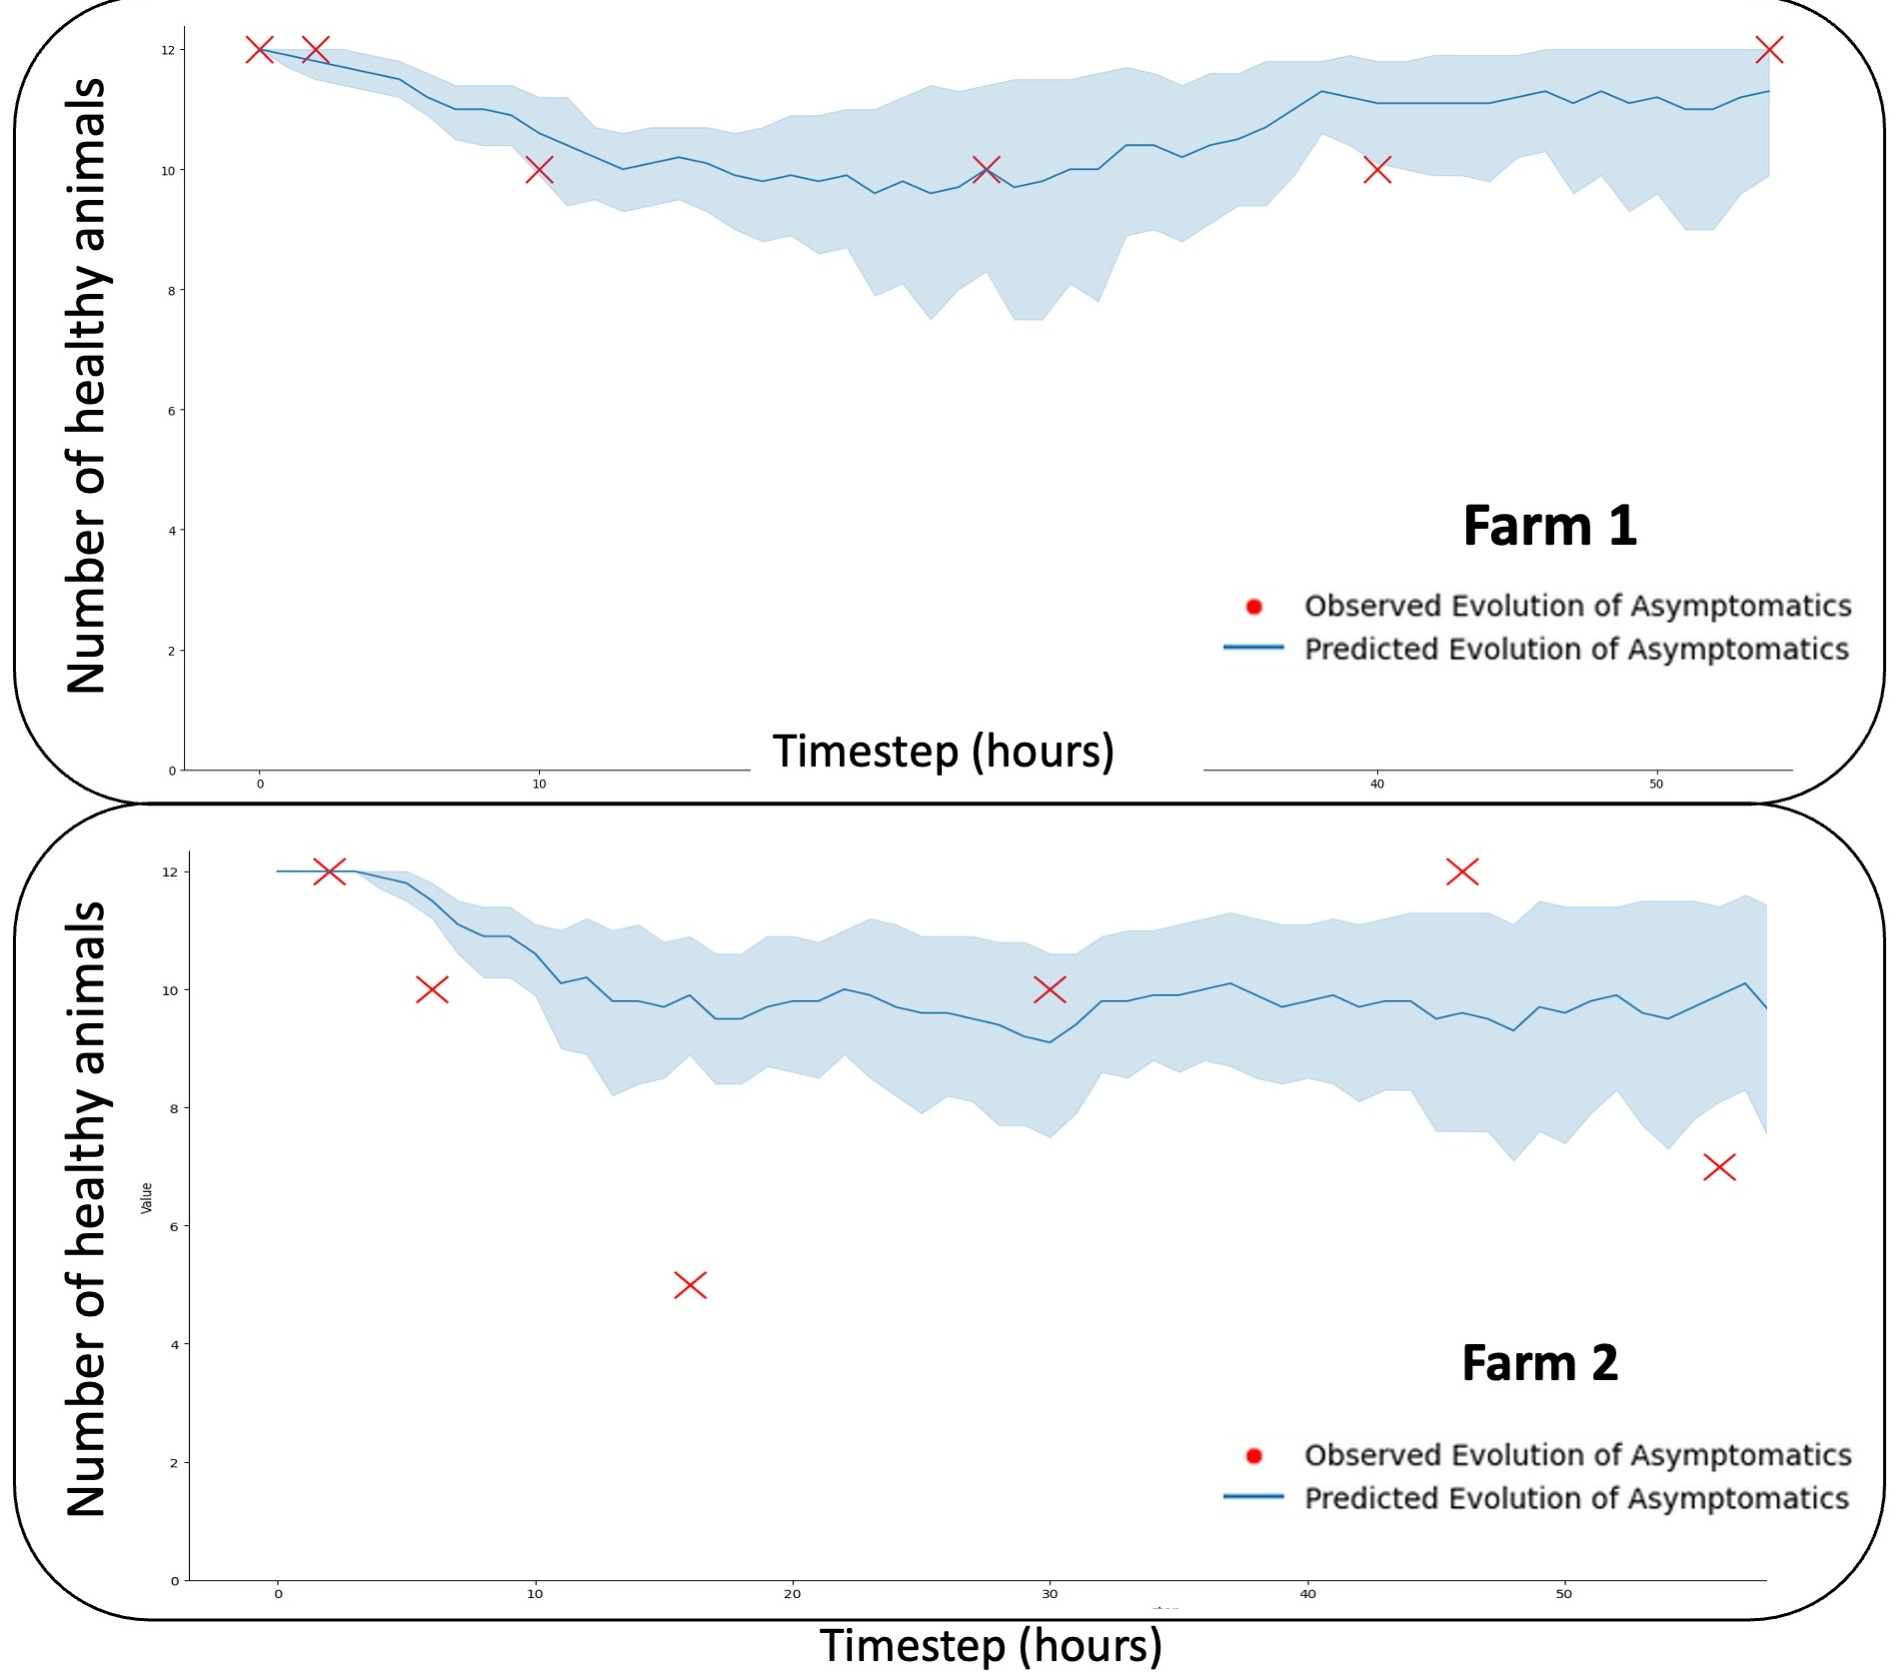
\includegraphics[width=\linewidth]{figures/chap2/prognosis-chap1.jpg}
      \caption{Asymptomatic forecast: ground truth vs predictions of an average pathogen mechanistic model}
      \label{fig:prognosis-chap1}
    \end{figure}

    \item A deep learning model based on a spatio-temporal CNN-RNN architecture was trained to classify animals’ clinical health status (symptomatic or asymptomatic) using pulmonary ultrasound videos. This model achieved an accuracy of approximately 72\% (table \ref{tab:feature_extractor_performance}). Specifically, the deep learning architecture combined convolutional neural networks (CNNs), serving as spatial feature extractors, and recurrent neural networks (RNN), which captured temporal information. Throughout the experiments, only the feature-extractor component—the CNN architecture—was varied, while the RNN architecture remained fixed across all tested models. The CNN's goal was to identify and extract relevant spatial features within individual ultrasound frames, such as lesions, pleura lines, or other anatomical details indicative of BRD. Conversely, the RNN aimed to leverage temporal sequences of these extracted features to model their evolution over the video duration. Different CNN architectures were evaluated, including EfficientNetB7, InceptionResnetV2, InceptionV3, VGG16, and an ensemble model combining InceptionV3 with InceptionResnetV2. Among these architectures, InceptionV3 achieved the highest performance, with a weighted F1-score of 70\%, precision of 72\%, recall of 69\%, and an overall accuracy of 69\%. In contrast, VGG16 demonstrated significantly lower performance, yielding an F1-score of only 14\%. The performance of the final selected deep learning model was assessed on two separate farms to verify its robustness and generalizability under contrasting practical conditions.
    
    \begin{table}[h]
        \centering
        \renewcommand{\arraystretch}{1.2} % Adjust row height for better readability
        \begin{tabularx}{\linewidth}{l *{4}{>{\centering\arraybackslash}X}}
            \toprule
            Feature Extractor & \small Weighted Precision & \small Weighted Recall & \small Weighted F1-score & \small Accuracy \\
            \midrule
            
            EfficientNetB7 & 0.67 & 0.62 & 0.63 & 0.62 \\
            InceptionResnetV2 & 0.71 & 0.50 & 0.49 & 0.50 \\
            InceptionV3 & \textbf{0.72} & \textbf{0.69} & \textbf{0.70} & \textbf{0.69} \\
            VGG16 & 0.09 & 0.31 & 0.14 & 0.31 \\
            InceptionV3 + InceptionResnetV2 & 0.71 & 0.62 & 0.63 & 0.62 \\
            
            \bottomrule
        \end{tabularx}
        \caption{Diagnosis performance of different deep learning architecture}
        \label{tab:feature_extractor_performance}
    \end{table}
    % \newpage 
        
\end{enumerate}

These results demonstrate the individual feasibility of both diagnostic automation using deep learning and epidemiological prognosis via mechanistic modelling. However, the two phases—diagnosis and prognosis—were not yet integrated into a complete predictive pipeline. Results highlighted the limitations of employing an average pathogen model universally, as BRD is intrinsically a multi-pathogen disease, and pathogen-specific variations significantly influence infection dynamics and disease severity. In the next chapter, methodologies for selecting the optimal prognosis expert model from multiple alternatives using outbreak observations will be discussed. 


% Pour ta thèse comme pour chaque chapitre, tu dois répondre à plusieurs questions impéra-tivement : 

% 1.	c'est quoi le problème ? (et dans quel contexte c'est un problème ?) à quelle question scientifique tu cherches à répondre ?

% 2.	en quoi c'est dur ?

% 3.	comment ça se positionne par rapport à l'existant : d'autres travaux / littérature (y compris par rapport à tes autres travaux pour le cas de chaque chapitre)

% 4.	quelles méthodes tu as employées, pourquoi, sous quelles hypothèses ?

% 5.	quels sont les résultats principaux ? en quoi ils apportent (ou pas) des éléments de réponse à la question (ou à d'autres questions) et quelles sont les questions qui se posent ensuite ?

% 6.	dans quelle mesure tes résultats sont-ils robustes ? quels sont les points faibles ou les limitations ? comment pourrait-on les corriger / contrebalancer (et est-ce nécessaire) ?

% 7.	enfin qu'est-ce qui resterait à explorer / faire ? quelles autres questions émergent à l'issue de ton travail ?

\subsection{[In French] Résumé grand public}

%-----------------------------------
%	SECTION 
%-----------------------------------

La maladie respiratoire bovine (BRD) est une pathologie fréquente et complexe qui représente un défi majeur en élevage, entraînant des pertes économiques importantes liées aux traitements, à la diminution des performances zootechniques et à une mortalité accrue. Afin de diagnostiquer cette maladie, les vétérinaires ont parfois recours à l’échographie pulmonaire, une méthode rapide, non invasive et réalisable directement à la ferme grâce à des appareils portables. Ces appareils, utilisés habituellement pour l'échographie reproductive chez les bovins, permettent d’examiner rapidement les poumons des animaux sans exposition à la radiation, contrairement à la radiographie ou au scanner. L’échographie pulmonaire peut identifier précisément et rapidement certaines lésions pulmonaires associées à la BRD, telles que la consolidation des lobes pulmonaires, les abcès ou encore les épanchements pleuraux. Ces lésions échographiques sont d’autant plus importantes qu’elles peuvent indiquer la gravité de la maladie, prédire les rechutes et renseigner sur les performances futures des animaux atteints.

Le projet SEPTIME, dans lequel s’inscrit ce travail de thèse, a permis la collecte de nombreuses données empiriques issues d’échographies pulmonaires enregistrées directement dans des élevages bovins durant les années 2023 et 2024. À partir de ces vidéos échographiques annotées par des vétérinaires experts, nous avons exploré deux approches complémentaires afin d’améliorer le diagnostic et le pronostic de la BRD :


\begin{enumerate} 
    \item L’utilisation de modèles d’intelligence artificielle (apprentissage profond) permettant d’automatiser rapidement la détection des cas cliniques de BRD à partir d’échographies pulmonaires. Ces modèles montrent un bon potentiel avec une précision atteignant environ 72\% dans la reconnaissance automatique de la maladie.

    \item Le paramétrage et l’évaluation d’un modèle mécaniste épidémiologique, qui simule la propagation à long terme de la maladie à partir d'observations réelles issues du terrain. Ce modèle mécaniste, une fois calibré, permet de prédire efficacement l’évolution de la maladie sur plusieurs semaines et pourrait ainsi aider les éleveurs à anticiper les épidémies et à adapter leurs stratégies de gestion sanitaire.

\end{enumerate}


Ces résultats démontrent la faisabilité individuelle de l'automatisation du diagnostic et du pronostic à l'aide de l'apprentissage profond et du pronostic épidémiologique via la modélisation mécaniste. Le chapitre suivant aborde les méthodologies de sélection du modèle expert de pronostic parmi de multiples alternatives en utilisant des observations cliniques.

\section{Proceedings published in Society for Veterinary Epidemiology and Preventive Medicine, 2024}

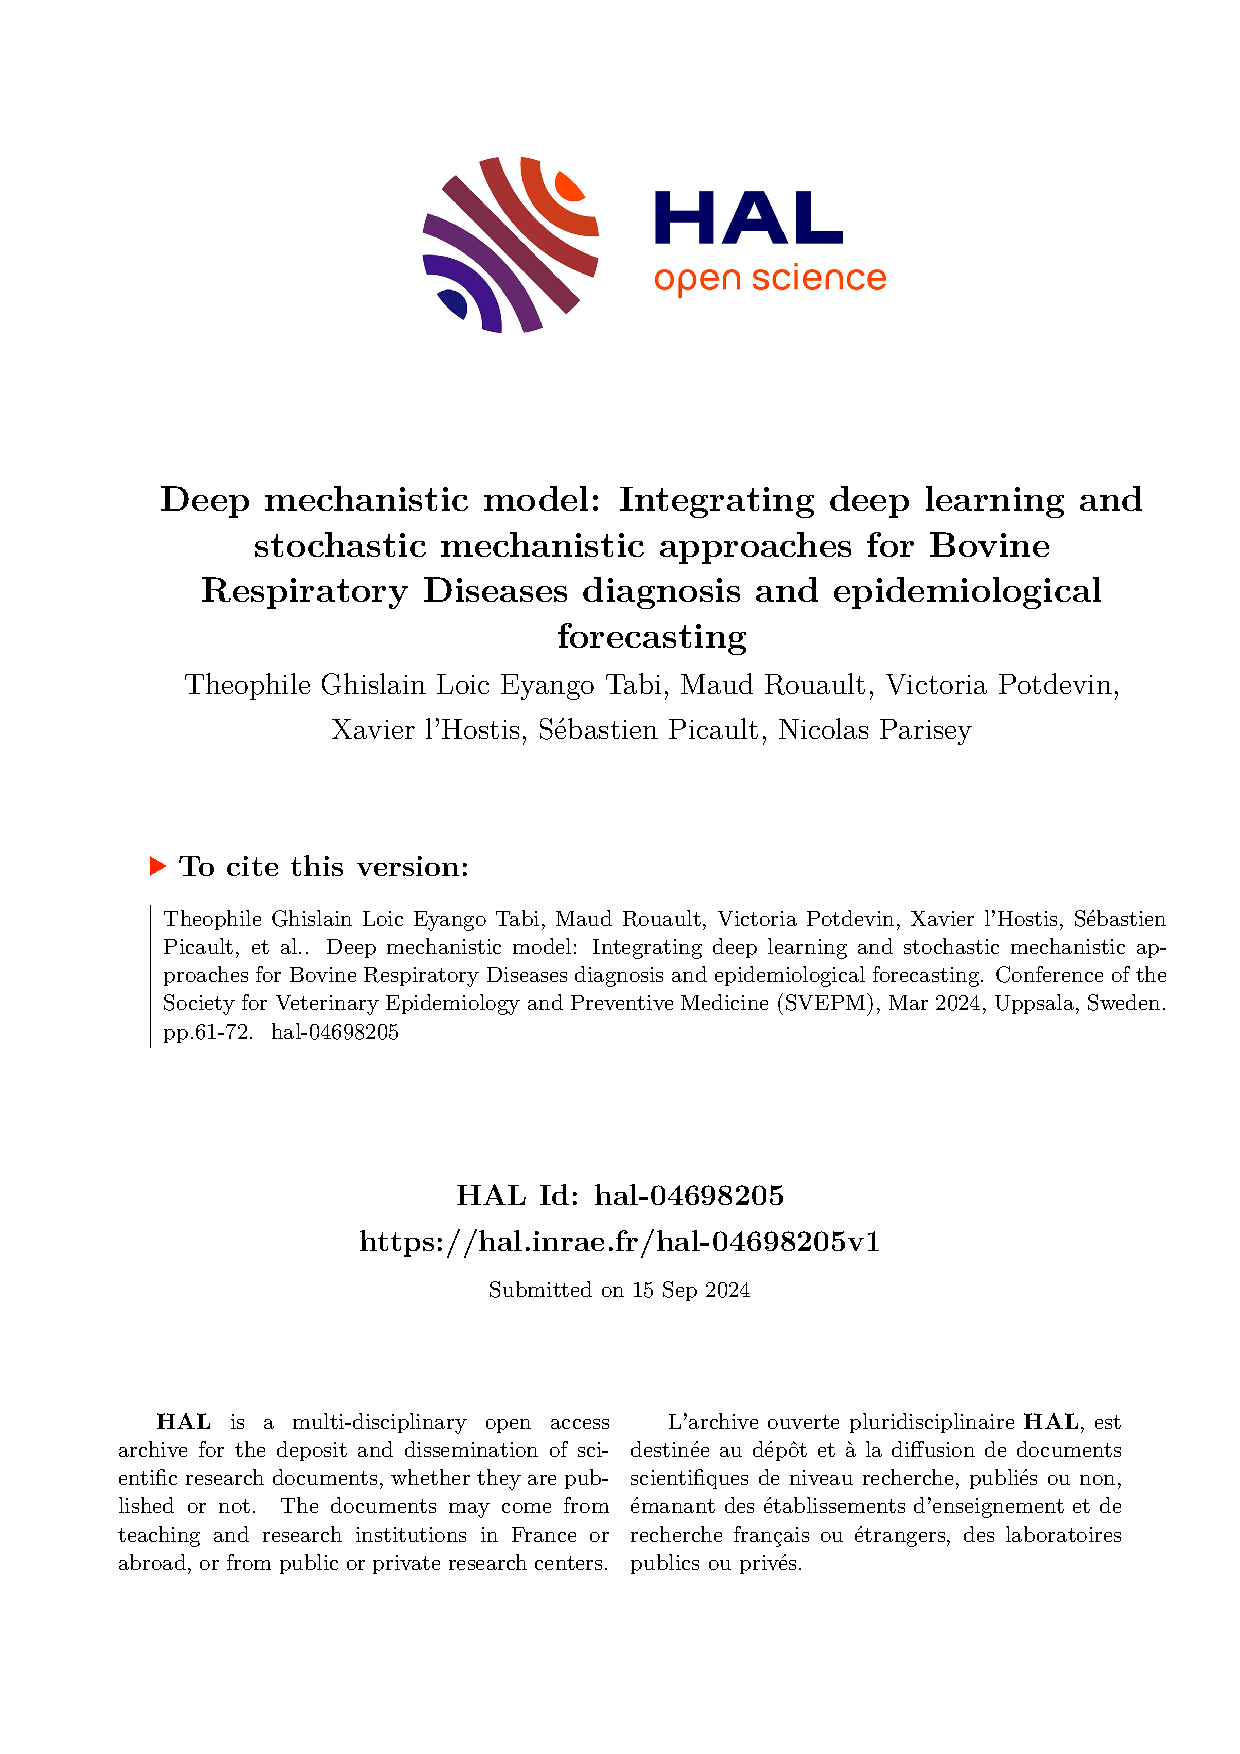
\includepdf[pages=-]{articles/SVEPM.pdf}  % Replace with your actual filename

